
\fullcite{modm02}

%-------------------
\begin{multicols}{2}
\begin{center}
{\bf Article excerpts}
\\ 
{\bf Notes and remarks}
\end{center}
\end{multicols}

\begin{multicols}{2}
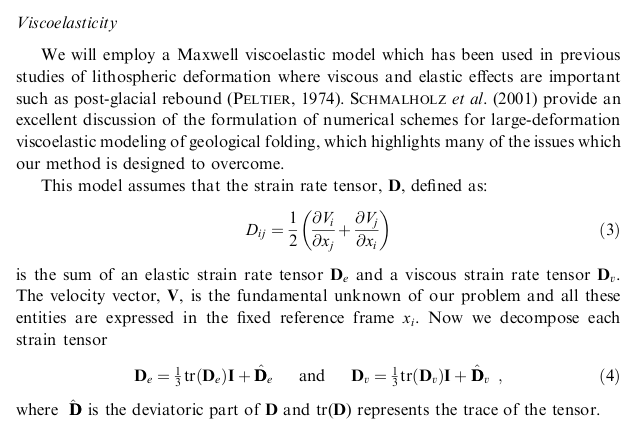
\includegraphics[width=8.25cm]{images/viscoelasticity/modm02a}\\
\[
\dot{\bm\varepsilon}=\frac12
(\vec\nabla \vec\upnu + \vec\nabla \vec\upnu ^T )
\]
\[
\dot{\bm\varepsilon}_e^d = 
\dot{\bm\varepsilon}_e  - \frac13 {\rm tr} (\dot{\bm\varepsilon}_e) {\bm 1} 
\]
\[
\dot{\bm\varepsilon}_v^d = 
\dot{\bm\varepsilon}_v  - \frac13 {\rm tr} (\dot{\bm\varepsilon}_v) {\bm 1} 
\]

\end{multicols}

\begin{multicols}{2}
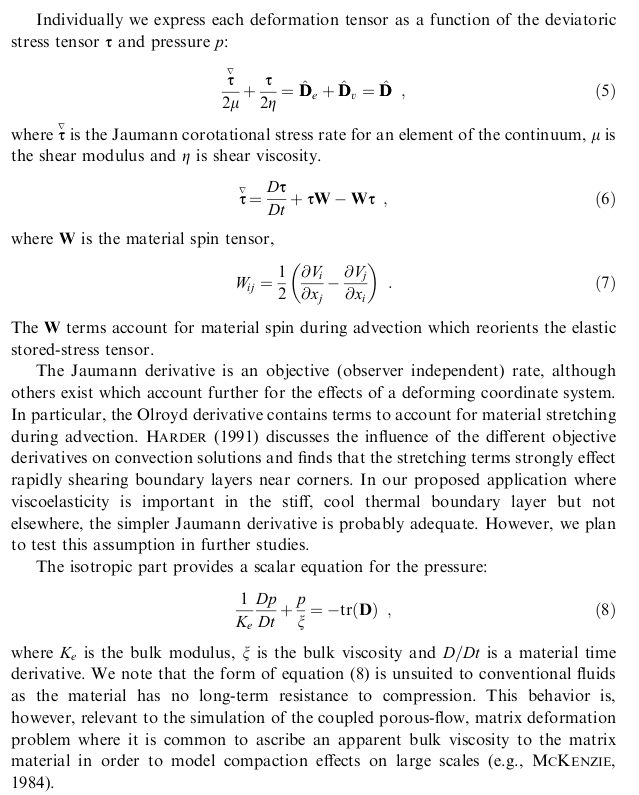
\includegraphics[width=8.25cm]{images/viscoelasticity/modm02b}\\
\[
\frac{TRIANGLE {\bm \tau}}{2 \mu}+\frac{{\bm \tau} }{2 \eta}
=
\dot{\bm\varepsilon}_e^d 
+
\dot{\bm\varepsilon}_v^d
=
\dot{\bm\varepsilon}^d 
\]
where 
$TRIANGLE {\bm \tau}$ is the Jaumann corotational stress rate
with 
\[
TRIANGLE {\bm \tau} = 
\frac{{\cal D}{\bm \tau}}{Dt} + 
{\bm\tau}\cdot {\bm\omega} - {\bm\omega}\cdot {\bm \tau}
\]


\[
\frac{1}{K} \frac{Dp}{Dt} + \frac{p}{\xi} = -{\rm tr}(\dot{\bm\varepsilon})
\]
\end{multicols}

\begin{multicols}{2}
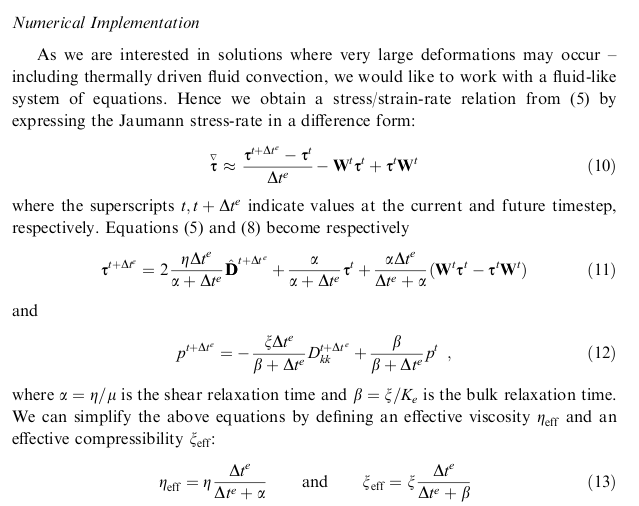
\includegraphics[width=8.25cm]{images/viscoelasticity/modm02c}\\
Numerical implementation
\[
TRIANGLE
\]
\end{multicols}

\begin{multicols}{2}
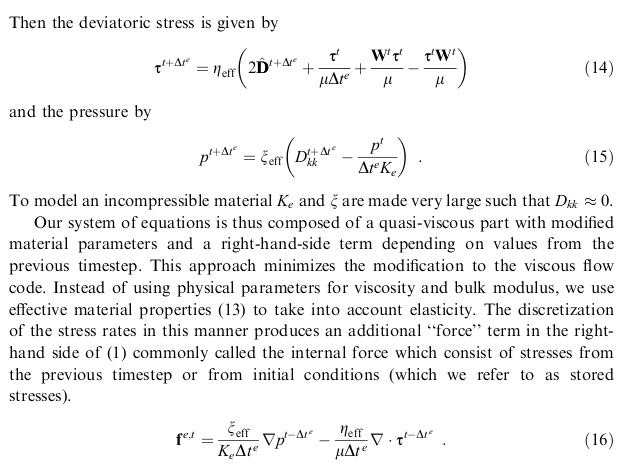
\includegraphics[width=8.25cm]{images/viscoelasticity/modm02d}\\
\end{multicols}

\begin{multicols}{2}
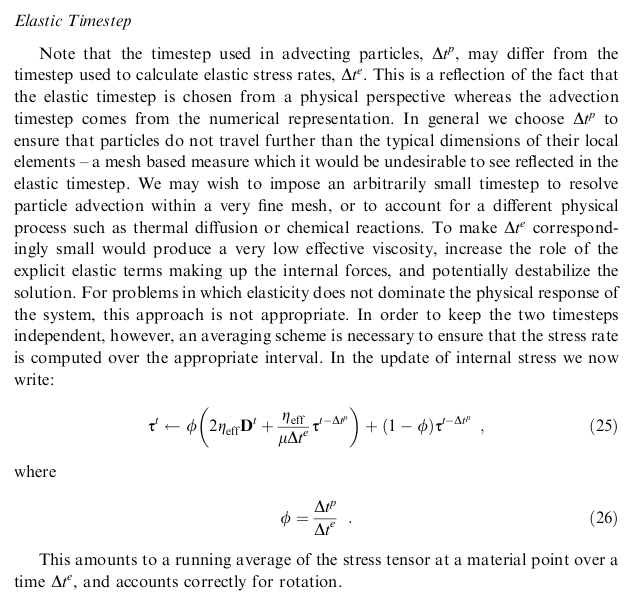
\includegraphics[width=8.25cm]{images/viscoelasticity/modm02e}\\
\end{multicols}

\begin{multicols}{2}
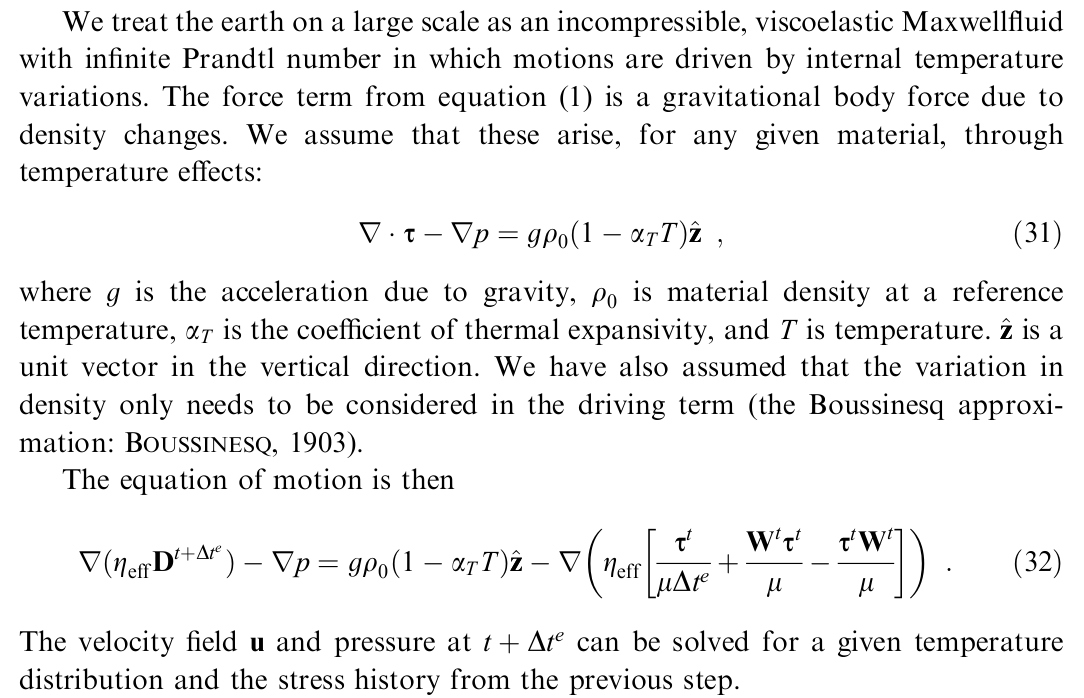
\includegraphics[width=8.25cm]{images/viscoelasticity/modm02h}\\
\end{multicols}







